% !TeX spellcheck = fr_FR
\documentclass[../main.tex]{subfiles}

\begin{document}

\subsection{Hawkes symétrique}

\begin{frame}{Expériences}
Dans le rapport $\rightarrow$ difficultés à apprendre des processus au moins multivariés $K\geq 2$.\pause

$\rightarrow$ Erratum dans le calcul de la vraisemblance (corrigé)

\textbf{Expérience 1} Processus de Hawkes bivarié symétrique (noyau exponentiel) sur $[0, 3600]$
\begin{itemize}
	\item $\alpha = \begin{bmatrix}0.1 & 0.01 \\ 0.01 & 0.1\end{bmatrix}$
	\item $\beta = 1$
	\item $\mu_1 = \mu_2 = \num{0.1}$
\end{itemize}
\end{frame}

\begin{frame}

\begin{figure}
	\includegraphics[width=\linewidth]{../results/intensity_baseHawkes2D.pdf}
	\caption{Intensité du processus de Hawkes, généré avec \texttt{tick}.}
\end{figure}
\end{frame}

\begin{frame}
\begin{figure}
\begin{subfigure}{\linewidth}
	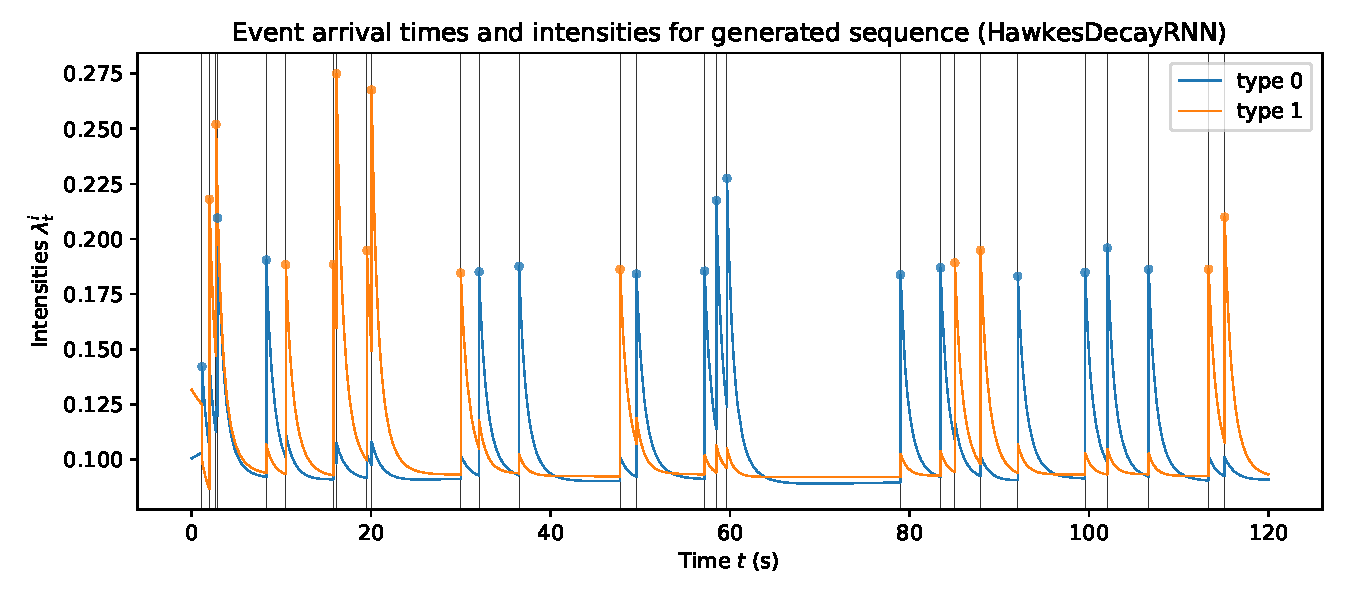
\includegraphics[width=\linewidth]{../results/intensity_HawkesDecayRNN_2d_hidden128_20181209-132014.pdf}
	\caption{Intensité et événements générés par le Decay-RNN calibré sur le Hawkes bivarié.}
\end{subfigure}
	\caption{Intensité apprise par le réseau RNN.}
\end{figure}
\end{frame}

\begin{frame}
\begin{figure}\ContinuedFloat
\begin{subfigure}{\linewidth}
	\includegraphics[width=\linewidth]{../results/intensity_HawkesDecayRNN_2d_hidden64_20181209-003122_OLD.pdf}
	\caption{Avec une erreur d'indice dans le calcul. Le réseau apprend à <<~écraser~>> les autres composantes de l'intensité après chaque événement.}
\end{subfigure}
\end{figure}
\end{frame}

\begin{frame}
\begin{figure}
	\centering
	\includegraphics[width=\linewidth]{../results/2D_Hawkes_Data_RMSE_20181209-181315.pdf}
	\caption{Résultats pour la prédiction d'événements, apprentissage sur des trajectoires d'un Hawkes bivarié ($K=2$).}
\end{figure}
\end{frame}

\begin{frame}
\begin{figure}
\begin{subfigure}{\linewidth}
	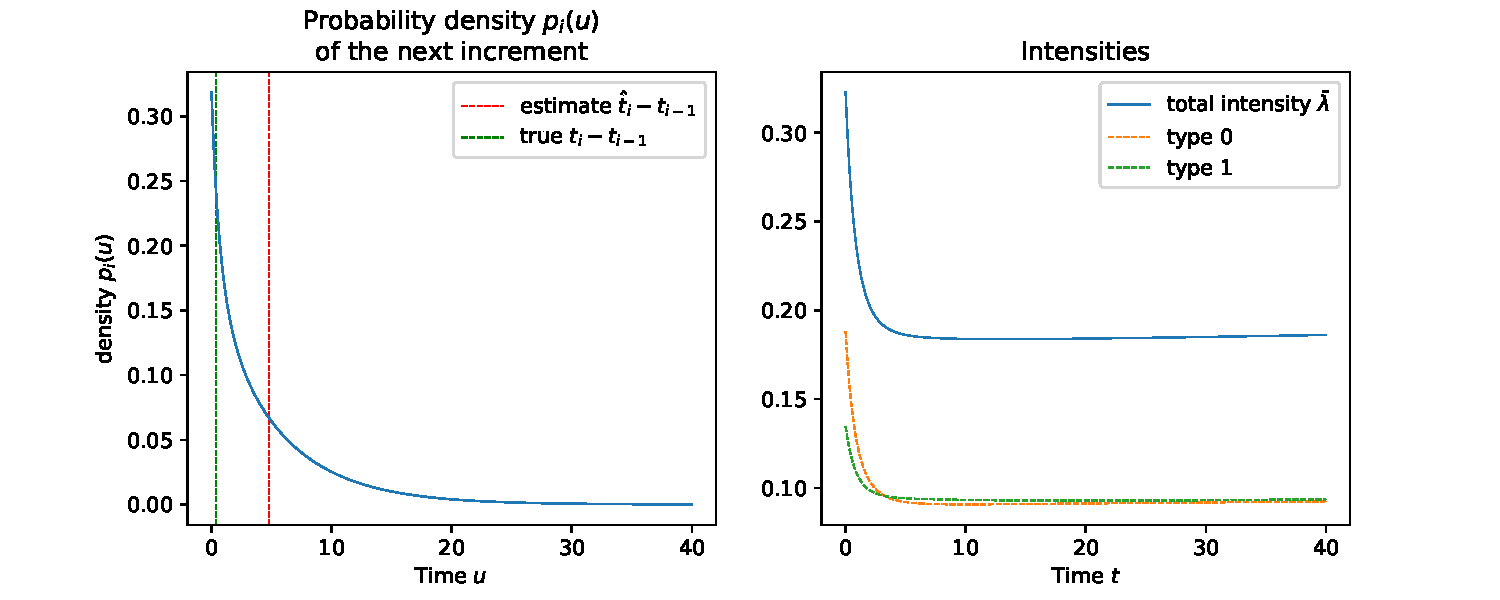
\includegraphics[width=\linewidth]{../notebooks/decayrnn_2d_prediction_graphs_hidden128_NEW.pdf}
	\caption{Le processus de Hawkes sous-jacent est symétrique: pour le prochain événement, les types sont équiprobables.}
\end{subfigure}
	\caption{Loi du temps du prochain événement, et intensités $(\lambda^i_t)_{t\geq t_{i-1}}$ de chaque type.}
\end{figure}
\end{frame}

\begin{frame}
\begin{figure}\ContinuedFloat
\begin{subfigure}{\linewidth}
	\includegraphics[width=\linewidth]{../notebooks/decayrnn_2d_prediction_graphs_OLD.pdf}
	\caption{Avec la faute de calcul. Le type du prochain événement est certainement celui du dernier.}
\end{subfigure}
\end{figure}
\end{frame}

\subsection{Hawkes asymétrique}

\begin{frame}
\textbf{Expérience 2} Processus de Hawkes asymétrique, $T = 1800$
\begin{itemize}
	\item $\alpha = \begin{bmatrix}0.1 & 0.07\\ 0.01 & 0.15\end{bmatrix}$
	\item $\beta = 1$
	\item $\mu_1 = \num{0.3} = 3\mu_2$
\end{itemize}
\end{frame}

\begin{frame}
\begin{figure}
	\includegraphics[width=\linewidth]{../results/intensity_baseHawkes2D_asymmetrical.pdf}
	\caption{Intensité du processus généré avec \texttt{tick}.}
\end{figure}
\end{frame}

\begin{frame}
\begin{figure}
	\includegraphics[width=\linewidth]{../results/intensity_HawkesDecayRNN_2d_hidden128_20181209-212603.pdf}
	\caption{Trajectoire générée par le Decay-RNN calibré sur le processus asymétrique.}	
\end{figure}
\end{frame}

\begin{frame}
\begin{figure}
	\includegraphics[width=\linewidth]{../results/intensity_HawkesLSTM_2d_hidden128_20181209-214506.pdf}
	\caption{Trajectoire générée par le LSTM.}
\end{figure}
\end{frame}

\begin{frame}
\begin{figure}
	\includegraphics[width=\linewidth]{../results/2D_Hawkes_Asymmetrical_Data_RMSE_20181209-221850.pdf}
	\caption{Résultats pour la prédiction d'événements, sur les données Hawkes asymétrique.}
\end{figure}
\end{frame}

\subsection{Application: mouvement de mid-price}

\begin{frame}{Application}

Le mid-price est donné par
\begin{equation*}
	P_t = \frac{P^\text{ask} + P^\text{bid}}{2}.
\end{equation*}

\textbf{Objectif} Modéliser les mouvements du mid-price

\begin{itemize}
	\item $N_t^{(a)}$ nombre d'augmentations
	\item $N_t^{(b)}$ nombre de baisses
\end{itemize}

On retrouve le mid-price par \autocite{2015arXiv150204592B}
\begin{equation}
	P_t = P_0 + N_t^{(a)} - N_t^{(b)}
\end{equation}

\end{frame}

\begin{frame}
\begin{figure}
	\begin{subfigure}{0.6\linewidth}
		\includegraphics[width=\linewidth]{../logs/loss_plot_HawkesLSTM-2d_hidden128-20181210-200505.png}
		\caption{Modèle LSTM.}
	\end{subfigure}
	\begin{subfigure}{0.6\linewidth}
		\includegraphics[width=\linewidth]{../logs/loss_plot_HawkesDecayRNN-2d_hidden128-20181210-200457.png}
		\caption{Modèle Decay-RNN.}
	\end{subfigure}
	\caption{Courbes d'entraînement sur le jeu de données DAX.}
\end{figure}
\end{frame}

\end{document}